\documentclass{article}
\usepackage[utf8]{inputenc}
\usepackage[T1]{fontenc}
\usepackage{url}

\usepackage[demo]{tikzpeople}
\begin{document}

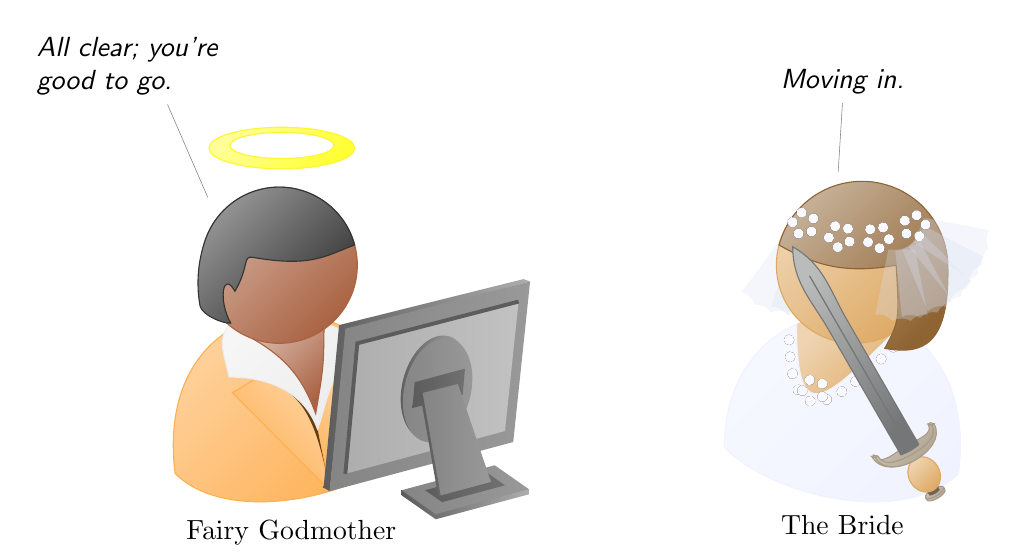
\begin{tikzpicture}[pin distance=1cm,every pin/.append style={font=\sffamily\itshape}]
\node[alice,good,monitor,minimum size=3cm,
pin={[text width=8em]95:{All clear; you're good to go.}}]
{Fairy Godmother};

\node[bride,sword,mirrored,minimum size=3cm,
pin={Moving in.}] at (7cm,0)
{The Bride};
\end{tikzpicture}

\vspace*{3cm}


\begin{tikzpicture}[pin distance=1cm,every pin/.append style={font=\sffamily\itshape}]
\node[santa,minimum size=2.5cm,
pin={Ho ho ho!},anchor=south]{};

\node[sailor,female,mirrored,minimum size=1.5cm,
anchor=south,pin={85:We've been good!}] at (6.25cm,0) {};
\node[charlie,mirrored,minimum size=1.5cm,
anchor=south] at (5cm,0) {};
\end{tikzpicture}

\bigskip

\definecolor{OverleafGreen}{RGB}{71,171,76}

\begin{tikzpicture}
\node[duck,minimum size=2cm,skin=OverleafGreen,hair=OverleafGreen] {};
\end{tikzpicture}

See the \texttt{tikzpeople} package documentation (\url{http://mirrors.ctan.org/graphics/pgf/contrib/tikzpeople/tikzpeople.pdf}) for other options.

\alltikzpeople{1.5}{}

\end{document}
